\chapter{Introduction}
\label{ch:intro}
\setcounter{page}{1}
\pagenumbering{arabic}

\section{Problem statement and motivation}
\label{sec:statement}
Over the past decade, we have witnessed a dramatic increase in the number of social Web applications. These applications come in different forms and offer different services such as social networks, content management systems (CMS), software forges, bug trackers, blogging tools, or collaboration services in general.\\

Since the launch of the first large social networking website in 1997~\cite{ellison2007social}, the social Web has seen a significant increase in its size and usage. Rather than simply consuming websites, users began to generate their own content through blogging tools and social networks, marking the start of Web 2.0 and the Semantic Web~\cite{berners1999weaving}. Social Websites have responded to this new trend by providing users with the ability to create their own personal profile where they could list friends, post photos, status updates and more. Later, some of these websites have also provided plug-ins that were used to integrate some of their social functionalities on other third-party websites. But what exactly is a social website and what functionalities do these websites offer to users? Is the ability to form a connection between users enough to consider a website to be a part of the social Web, and how can we expect the social Web to evolve in the future?\\

In this thesis we will analyse and propose means to achieve data ownership and interoperability for decentralized social Web applications, with respect to privacy and access control. Since the user's data are such an important asset of the current business models for most social Websites, companies have no incentive to share data among each other or to offer users real ownership of their own data in terms of control and transparency of data usage. We have concluded therefore that it is important to improve the social Web in such a way that it allows for viable business models while still being able to provide increased data ownership and data interoperability compared to the current situation.\\

The following section of the introduction outlines the reasons and the motivation that has driven us to pursue this thesis. The first topic discusses the lack of control over users' data. The second topic covers identity, as a key factor for the decentralized social Web. Finally, the third topic will be an introduction to achieving interoperability on the Web.

\subsection{Data silos, losing control over our data}
\label{subsec:intro-silos}
A current practice specific to most Web services is to centralize user resources, becoming the so-called "data silos". Often when adhering to particular services we usually end up creating dedicated local accounts, which ties and limits us to a particular service and/or resource. Figure~\ref{fig:wall_garden} aptly illustrates this aspect, depicting how people's freedom within a particular social networking site is limited and how they would like to "jump out of the walled gardens" to interact with "other" social networking sites, such as to share their data with their friends who may be members of other social networking sites. Furthermore, users have no control over how their personal account data are used by applications, as it is the case for private data that is often sent to third party companies for advertising purposes.

\begin{figure}[h]
  \begin{center}
    \includegraphics[width=300px]{img/walled_garden.jpg}
        \caption{'Everywhere and nowhere', an illustration by David Simonds, 2008.}
        \label{fig:wall_garden}
  \end{center}
\end{figure}

One may argue that better privacy policies may reduce the risk of exposure. However, even if users decide to protect their public data through rigorous privacy settings, or even remove their accounts, there is no guarantee that the process is instant and more importantly, permanent. This is mainly due to the fact that countries have passed laws forcing online services to store user data for several months up to one year or an unlimited period of time.\\

Companies attempt to justify the practice of \textit{data silos} stating that they have better control over user actions while allegedly offering better security. Online businesses stand to gain a lot from data mining their users in order to be able to increase their sales, or offer targeted publicity. In most of the cases, they offer "free" sign-up for their services and provide people with numerous attractive features, encouraging them to provide additional personal data, effectively turning the users from customers into products which are often "sold" to third party advertising companies. For this matter and to the detriment of users, privacy is often found as an additional feature and it is not implemented by design.\\

While it is true that some people join public communities and disclose personal information in order to find new friends who share common interests, others would simply want to have more control over their privacy. The situation worsens when social networks force the users into providing their real names without presenting them with alternatives, like creating multiple identities or using pseudonyms.\\

A solution to the so-called \textit{data silos} can be achieved through decentralization, where users are free to host their data wherever they want. In the following section we will discuss how decentralized identity systems play an important role in achieving true data ownership for users.


\subsection{Identity, a key factor for the decentralized social Web}
\label{subsec:intro-id}
Before discussing decentralized social Web applications, we must first define the concept of \textit{identity}. The first question we ask ourselves is related to the form and nature of online identities. Often, an online identity starts with a unique identifier binding a person to a user profile describing them. The identity of a person may also include the sum of all opinions and postings that have been generated by that person, as well as relationships between the person and other people, all contributing to the one's reputation.\\

Since online identities also deal with personal data, a number of risks are related to the exposure of these data~\cite{rosenblum2007}. There have been accounts of employers who have been collecting information about potential employees from their blogs~\cite{viegas2005bloggers} and social networking sites~\cite{mannan2008privacy}, and have used this information to dismiss them or deny them jobs. A recent study~\cite{careerbuilder2009} performed by a popular career and resume-building website revealed that 46\% of executives say they are likely to make a hiring decision based on a prospective employee's online identity or Facebook profile. So far, the most common workaround for people has been to replace real identities with pseudonyms.\\

Identity is easily one of the most difficult research areas on the Web, as it requires both practical solutions and multidisciplinary research. We believe that identity implies to be able to refer reliably to anything, abstract or real, and in different contexts. In our day to day lives, we find the concept of personal identity to be quite simple (i.e. our names). Yet on closer inspection, we find that applying these concepts to a Web scale becomes quite tricky, as is the case when we type our name into a search engine and see that it may refer to many other people in different contexts. It becomes even worse when it might refer to us in a context that we did not intend to.\\

One way to deal with identity is to establish a common convention that identifies particular things in a uniform manner that is 
easily reused in diverse contexts. When applied to the Web, it becomes obvious that using HTTP Uniform Resource Identifiers (URIs) as global identifiers is the preferred choice. The key advantage of HTTP URIs over any other identification scheme (e.g. email addresses, unique user IDs, etc.) is that linked data principles say these URIs should return a useful description of what the URI identifies when accessed in a Web browser or computer application using the HTTP protocol.\\

The process of establishing one's identity leads to \textit{identification}, which is also a key component of decentralized social Web services. Having a persistent identity across different application domains is very difficult to achieve, since the concept of \textit{decentralized authentication} requires a considerable effort from large entities in terms of compatibility, as well as powerful trust relationships between all parties. Many services authenticate users based on user name and password combinations, which results in having to remember and manage a lot of accounts. In that respect, federated and decentralized authentication services like OpenID~\cite{recordon2006openid}, OAuth~\cite{hardt-d-2012-a} and Mozilla Persona~\cite{browserid} have proven to be quite useful. However, once the authentication has been performed, some services still require that users have local accounts in order to manage profile data. To this regard, WebID, the first of our contributions, provides both a decentralized identity platform, as well as the basis for a deceptively simple yet secure decentralized authentication mechanism through the use of cryptography, in the form of WebID-TLS. WebID and WebID-TLS will be presented in detail in Chapter~\ref{ch:identity}.

\subsection{Interoperability based on the Semantic Web and LDP}
\label{sec:semweb}
A decentralized Web application must be able to work \textbf{across different application domains}, enabling different applications to interact with each other through the use of data semantics. It is important that users be allowed to choose where to store their data, may that be on personal servers they own and keep in their homes, or entrusting their data to their friends or people they trust. Users may even take advantage of a myriad of cloud storage services available on the Web, though steps must be taken to ensure the privacy of their data, with respect to the service providers.\\

The main cause for which storing data in a decentralized manner is unpopular, is that major Web services have no incentive to share data among each other or to give users more ownership than necessary for their own data. Even though most applications provide Application Programming Interfaces (APIs) which are dedicated to performing specific interoperability tasks, developers are still required to have a priori knowledge of these APIs before attempting to provide interoperability. To our knowledge, there is currently no standardized API for decentralized Web applications, leaving at the discretion of each application to define its own API. Recently however, a standard is being proposed for such an API within the World Wide Web Consortium (W3C). It relies on the \textit{Semantic Web}, which refers to the Web of data~\cite{berners1999weaving}, in order to offer true interoperability.

\subsubsection{The Semantic Web}
The Semantic Web should be considered in some ways like a global database, or better yet an information space. Since most of the information on the Web is designed for human readers, though only useful for human-to-human interaction, the Semantic Web intends to allow machines to participate in this interaction by providing languages for expressing information in a machine processable form. In other words, the Semantic Web offers the tools to convey the meaning of data so that it will be understood by computers and not misinterpreted.\\

The most common means used by the Semantic Web to describe information are the Resource Description Framework (RDF)~\cite{klyne2004resource} and the Turtle~\cite{beckett2008turtle} syntax. While RDF is based upon the idea of making statements about resources (in particular Web resources) in the form of subject-predicate-object expressions (called \textit{triples}), the Turtle syntax is utilized to express data in the RDF data model.\\

A typical triple is presented in Example~\ref{ex:semweb}, where the subject is \verb+<>+ (which refers to the current document), the predicate is \verb+foaf:maker+ while the object being \verb+https://barry.example/profile#me+. All statements are contained within the same document, residing at \verb+https://barry.example/profile+, and having as \textit{primaryTopic} the inner reference \textbf{\textit{\#me}} pointing to a \textit{Person}, namely Barry. A visual representation of the same triples is provided as a graph in Figure~\ref{fig:intro-foaf}.\\

\begin{example}
\begin{minted}{turtle}
@prefix foaf: <http://xmlns.com/foaf/0.1/> .

<> a foaf:PersonalProfileDocument ;
      foaf:maker <https://barry.example/profile#me> ;
      foaf:primaryTopic <https://barry.example/profile#me> .

<#me> a foaf:Person ;
      foaf:name "Barry" ;
      foaf:knows <https://example.edu/p/Ann#MSc> ;
      foaf:weblog <http://barry.example/blog> .
\end{minted}
\caption{A typical subject-predicate-object relation in Turtle.}
\label{ex:semweb}
\end{example}

\begin{figure}[htbp]
  \begin{center}
    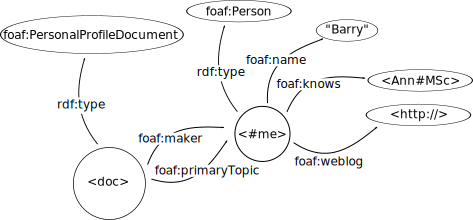
\includegraphics[width=300px]{img/foaf-ontology.pdf}
        \caption{A graph representation of Barry's profile.}
        \label{fig:intro-foaf}
  \end{center}
\end{figure}

The Semantic Web facilitates cross-domain applications and services, thanks to data being structured into ontologies and vocabularies. An ontology formally represents knowledge as a set of concepts within a domain, and the relationships between those concepts. Vocabularies are a less formal way of expressing concepts or entities and the relations between them. A typical case of a large linked data application is DBPedia\footnote{http://dbpedia.org}, which, essentially, makes the content of Wikipedia available in RDF. The importance of DBPedia is not only that it includes Wikipedia data, but also that it incorporates links to other datasets on the Web, e.g., to Geonames\footnote{http://geonames.org}. By providing extra links expressed as RDF triples, applications are able to exploit the semantics of data and gain additional knowledge from other datasets. Conversely, by virtue of integrating facts from several datasets, applications are now able to provide a better user experience.\\

\subsubsection{The Linked Data Platform}
The \textbf{Linked Data Platform} (LDP)~\cite{ldp2013} is considered to be the first attempt at producing a standardized API for Web applications. Essentially, it is a set of best practices for a read-write Linked Data architecture, based on HTTP access to Web resources that describe their state using the RDF data model. It describes the use of HTTP verbs for fetching (GET), updating (POST/PATCH), creating (PUT) and deleting (DELETE) resources from servers that expose their resources as Linked Data. It provides several rules as well as clarifications and extensions of the four rules of Linked Data, which are the following:

\begin{enumerate}
  \item Use URIs as names for entities;
  \item Use HTTP URIs so that people can look up those names;
  \item When someone looks up a URI, provide useful information, using existing standards (e.g. RDF, SPARQL);
  \item Include links to other URIs so that more information can be discovered.
\end{enumerate}

Adopting LDP is important since developers no longer have to redefine APIs every time a new Semantic Web application is created.\\

LDP focuses on two important concepts, \textbf{resources} and \textbf{containers}.\\

\textbf{Linked Data Platform Resources} (LDPRs) are HTTP resources that comply to the simple patterns and conventions in this section. HTTP requests to access, modify, create or delete LDPRs are accepted and processed by LDPR servers. Most LDPRs are domain-specific resources that contain data for an entity in some domain, which could be commercial, governmental, scientific, religious, or other.\\

\textbf{Linked Data Platform Containers} (LDPCs) are collections of LDPRs, similar to how blog posts are grouped into blogs, wiki pages are grouped into wikis, and products are grouped into catalogues. Example~\ref{ex:ldpc} describes a container and its resources.\\

\begin{example}
\begin{minted}{turtle}
@prefix dcterms: <http://purl.org/dc/terms/> .
@prefix rdfs: <http://www.w3.org/2000/01/rdf-schema#> .
@prefix ldp: <http://www.w3.org/ns/ldp#> .

<> a ldp:Container;
   dcterms:title "A very simple container" ;
   rdfs:member <member1>, <member2>, <member3> .
\end{minted}
\caption{A simple container represented in Turtle.}
\label{ex:ldpc}
\end{example}

In the next section, we briefly present the list of our contributions, with an in-depth discussion to follow in the next chapters.

\section{Main contributions}
\label{sec:intro-contrib}

\subsection{WebID}
A global distributed social Web requires that each person must be able to control their identity, that this identity be linkable across sites - placing each person in a Web of relationships - and making it possible to authenticate globally with such identities.\\

A \textbf{WebID}~\cite{webid2013} is an HTTP URI which uniquely refers to an Agent (Person, Organization, Group, Device, etc.). A description of the WebID can be found in the \textit{profile document}, a type of Web page that any Web user is familiar with, and which uses a standardized RDF serialization format. WebID uses vocabularies such as Friend-of-a-Friend (FOAF)~\cite{foaf} to provide a complete user profile, which is under the user's control~\cite{sambra2011myprofile}.\\

WebIDs can also be used to build a Web of trust by allowing people to link together their profiles in a public or protected manner~\cite{sambra2011friending}. Such a Web of trust can then be used by a Web application to make authorization decisions, by allowing access to resources depending on the properties of an agent, such that he/she is known by some relevant people, works at a given company, is a family member, is part of several groups, etc..\\

WebID is a work-in-progress open standard within the World Wide Web Consortium\footnote{http://w3.org}, for which I am one of the authors and also an editor. More information about WebID will be presented in Chapter~\ref{ch:identity}.

\subsection{WebID Authentication}
The \textbf{WebID-TLS}~\cite{webid-tls} protocol enables secure, efficient and user friendly authentication on the Web, by taking advantage of WebID and the TLS protocol~\cite{allen1999tls}. It enables people to authenticate to any site by simply clicking on one of the certificates proposed to them by their browser. These certificates can be created in one click by any WebID provider for their users.\\

The WebID-TLS protocol specifies how a Web application can authenticate a user after requesting his \textit{certificate} without requiring the certificate to be signed by a well known Certificate Authority. It relies on client certificates to prove that an agent possesses the private key that matches a public key stored in the WebID profile document. This also implies that only the owner of the private key has write access to the profile document and thus it is capable of adding an RDF description of his/her public key.\\

WebID-TLS authentication can also be used for automatic authentication by robots, such as Web crawlers of linked data repositories, which could be agents working on behalf of users to help them in their daily tasks. The WebID-TLS protocol is not limited to authentication on the World Wide Web, but can in theory work with any protocol based on TLS.\\

WebID-TLS \textit{access delegation}~\cite{tramp2012extending} is an important feature when applied to decentralized applications, as it no longer requires the user's presence when making authenticated requests. We have provided a solution that protects user privacy by allowing servers to respond to requests as if they were being made by specific users, and thus serving content based on the access control policies that are specific for the requesting user.

WebID-TLS is a work-in-progress open standard within the World Wide Web Consortium\footnote{http://w3.org}. We have contributed to the technical aspects of the specification over the past two years, and I am also one of its editors.  More information about WebID-TLS will be presented in Section~\ref{sec:webid-auth} of Chapter~\ref{ch:identity}.

\subsubsection{Extending the WebID-TLS protocol}

Based on WebID-TLS, we propose our third contribution, a mechanism that enables delegated authentication. This mechanism is useful especially for service providers that are not capable to deploy a local WebID verification service, and thus have to rely on a third party service to act as a WebID verifier. Section~\ref{sec:webid-tls_delegated_auth} of Chapter~\ref{ch:identity} offers a full description of this mechanism.\\

Access delegation is an important feature when applied to decentralized applications, as it no longer requires the user's presence when making authenticated requests. We hereby offer a solution that protects user privacy by allowing servers to respond to requests as if they were being made by specific users, and thus serving content based on the access control policies that are specific for the requesting user. More information about our forth contribution can be found in Section~\ref{sec:webid-delegated-access} or Chapter~\ref{ch:identity}.


\subsection{Social Access Control Service}
Our third contribution. the Social Access Control Service (SACS) is comprised of two distinct sub-services, a \textit{Relationship Monitor} (RM) engine and a \textit{Static Access Control} (SAC) engine, each having its own particular set of tasks (Section~\ref{sec:sacs} of Chapter~\ref{ch:ac}). SACS uses \textit{context} and \textit{social proximity distance} as metrics for access control policies~\cite{sambra2012context}.\\

The Social Access Control Service is especially useful for controlling personal user information, which is often prone to changes (e.g. status messages, phone numbers, list of friends, etc.). To achieve a user-friendly yet robust and flexible access control mechanism, as opposed to controlling access by separating users into groups, we decided to take advantage of a common social practice, namely the use of \textit{context}. Context labels are assigned to both profile information data (e.g. name, phone numbers, blog addresses, etc.) as well as to Web resources (e.g. photos, comments, etc.). The same labels will be assigned to users, in such a way that users labelled with a specific context (i.e. "work") can easily be matched against resources sharing the same context. \\

More information on access control will be provided in Chapter~\ref{ch:ac}.

\section{Thesis structure}
\label{sec:intro-summary}
The thesis is structured as follows. This chapter provides the motivation behind our research, as well as a short introduction to our contributions.\\

Chapter~\ref{ch:identity} describes our first four contributions. The first contribution, \textit{Web Identity and Discovery} (WebID), a simple and universal identification mechanism that is distributed and openly extensible. It improves privacy, security and control over how each person can identify themselves. The second contribution, the WebID-TLS authentication protocol, enables secure, efficient and user friendly authentication on the Web by allowing people to login using client certificates and without relying on Certification Authorities. The third and fourth contributions are an extension of WebID-TLS, offering delegated authentication and access delegation.\\

Chapter~\ref{ch:ac} presents our fifth contribution, a Social Access Control Service for Web applications. We begin by taking a detailed look at \textit{social context} and \textit{social proximity}, as metrics for a dynamic access control system tailored for social Web applications. When applied to the Social Access Control Service, these metrics contribute to the system's adaptability in terms of the dynamics of human relationships.\\

All our implementation efforts are presented in Chapter~\ref{ch:implementations}, as means to validate our research. This chapter contains all practical aspects of implementing a decentralized social Web, including identity, authentication, access control and data ownership. We introduce the project \textit{MyProfile}, which aims to be a decentralized identity provider. Next, we present two open source libraries (WebIDauth and WebIDDelegatedAuth) that are used to perform WebID-TLS authentication. Lastly, we describe RWW.I/O, a personal data store where different applications can store data about and for the user, and where data are equally available between applications.\\

Finally, Chapter~\ref{ch:conclusions} summarizes our research results by providing conclusions as well as a reflection on what we can do to improve our contributions and to provide new research directions. As part of the perspective work, we talk about the \textit{Semantic Messaging and Notifications Protocol} (SMNP) which intends to offer two distinct types of messages. The first type is similar to email, in that it provides end-to-end communication between the involved parties, while the second type consists of activity streams (i.e. updates about other users). We also discuss the possibility of creating a transparent WebID proxy, which uses certain parts of a user's WebID profile in order to build new identities specific to different types of services (e.g. anonymous, shopping, blogging, etc.).